\documentclass[11pt,a4paper,oneside]{article}
\usepackage{hyperref}
\usepackage{graphicx}


\author{Louis Bodnar}
\title{Urban Science Infographic Generator}
\begin{document}
\begin{titlepage}

\begin{center}

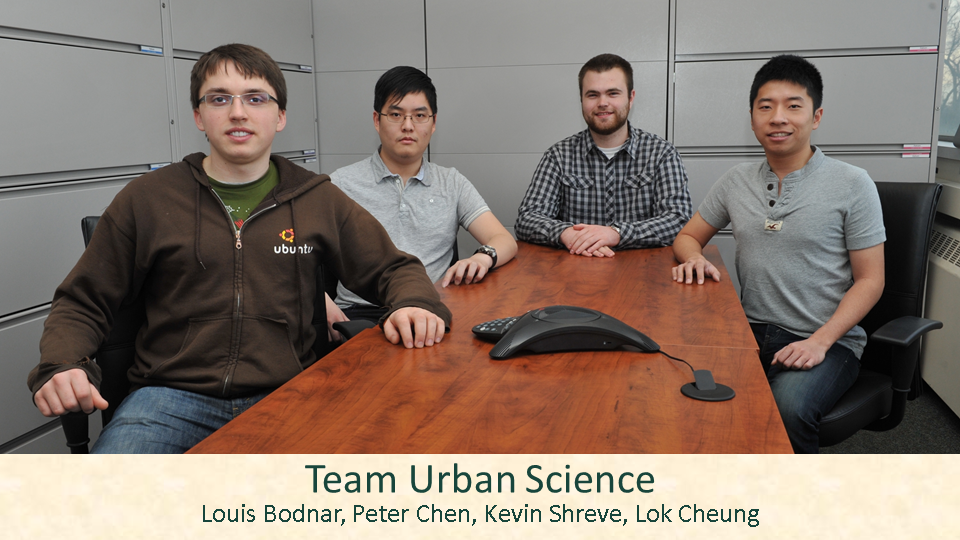
\includegraphics[width=1\textwidth]{./group_photo.png}\\[1cm]    

\textsc{\LARGE Team Urban Science}\\[1.5cm]

{ \huge \bfseries Infographic Generator}\\[0.4cm]

Louis Bodnar\\
Peter Chen\\
Lok Cheung\\
Kevin Shreve\\

\vfill

{\large \today}

\end{center}

\end{titlepage}


\tableofcontents

\section{All-Hands Meetings}
01/09: Capstone Overview\\
01/11: Project Plan\\
01/16: (Martin Luther King Day, No Meeting)\\
01/18: Risks and Prototypes\\
01/23: Team Team Status Report Presentations\\
01/25: Schedule and Team Work\\
01/30: Team Project Plan Presentations\\
02/01: Team Project Plan Presentations\\
02/06: Team Project Plan Presentations\\
02/08: Team Project Plan Presentations\\
02/13: Resume Writing and Interviewing\\
02/15: Creating and Giving Presentations\\
02/20: Team Alpha Presentations\\
02/22: Team Alpha Presentations\\
02/27: Team Alpha Presentations\\
02/29: Team Alpha Presentations\\
03/05: (Spring Break, No Meeting)\\
03/07: (Spring Break, No Meeting)\\
03/12: Design Day and the Project Video\\
03/14: Camtasia Demo\\
03/19: Team Status Reports\\
03/21: Team Status Reports\\
03/26: Team Status Reports\\
03/28: Team Status Reports\\
04/02: Team Beta Presentations\\
04/04: Team Beta Presentations\\
04/09: Team Beta Presentations\\
04/11: Team Beta Presentations\\
04/16: Ethics and Professionalism\\
04/18: Intellectual Property\\
04/23: Team Project Videos\\
04/25: Team Project Videos and All Deliverables\\
04/26: Team Design Day Setup\\
04/27: Team Design Day\\
05/01: Team Project Videos\\


\section{Project Summary}
\begin{itemize}
\item Functionalities
  \begin{itemize}
  \item Visualize Data and Information
    \begin{itemize}
    \item Graphically
    \item Compactly
    \item Creatively
    \end{itemize}
  \item Based on Key Performance Indicators (KPIs)
  \end{itemize}
\item Features
  \begin{itemize}
  \item Dynamic User Selections
    \begin{itemize}
    \item Key Performance Indicators
    \item Timeframes
    \end{itemize}
  \item Display Engaging Graphics
    \begin{itemize}
    \item Scalable
    \item Varied
    \end{itemize}
  \item Support Drill Down into KPIs
  \end{itemize}
\item Technologies
  \begin{itemize}
  \item Microsoft C\#/.NET, ASP.NET
  \item JavaScript
  \item CSS, HTML5
  \item SQL Server
  \end{itemize}
\end{itemize}



\section{Major Milestones}

\subsection{Status Report Presentations}
\textbf{Due: January 23, 2012}\\
\subsubsection{Assignment}
Each team gives a five minute status report on a variety of things including client contact, client meeting schedules, team meeting schedules, team organization, server systems and software, development systems and software, a brief description of the project, the status of their project plan, and the initial identification of risks.\\

A PowerPoint template is provided on the \href {http://www.cse.msu.edu/~cse498/2012-01/other-links/downloads}{Downloads} page.\\

As with all of these milestones, this date indicates the due date. So, in this case the due date is the Monday of the third week, which means that the teams have to complete this work in first three weeks.\\
\subsubsection{Deliverable}
\begin{itemize}
\item Project Description
  \begin{itemize}
  \item infographic generator
  \item HTML5 webapp
  \item generates infographics based on information from a database
  \item Description Point 4
  \end{itemize}

\item Project Plan Document
  \begin{itemize}
  \item Status Point 1
  \item Status Point 2
  \item Status Point 3
  \item Status Point 4
  \end{itemize}

\item Server Systems / Software
  \begin{itemize}
  \item Description \&/or Status Point 1
  \item Description \&/or Status Point 2
  \item Description \&/or Status Point 3
  \end{itemize}

\item Development Systems / Software
  \begin{itemize}
  \item Description \&/or Status Point 1
  \item Description \&/or Status Point 2
  \item Description \&/or Status Point 3
  \end{itemize}

\item Client Contact
  \begin {itemize}
  \item Had a conference call with our customer
  \item Set up weekly conference call times to talk about progress
  \end{itemize}

\item Team Meetings
  \begin{itemize}
  \item Set up meetings on Tuesday and Thrusday
  \item Status Point 2
  \end{itemize}

\item Team Organization
  \begin{itemize}
  \item Description Point 1
  \item Description Point 2
  \end{itemize}

\item Risks

\item Risk 1
  \begin{itemize}
  \item Description
  \item Mitigation
  \end{itemize}

\item Risk 2
  \begin{itemize}
  \item Description
  \item Mitigation
  \end{itemize}

\item Risk 3
  \begin{itemize}
  \item Description
  \item Mitigation
  \end{itemize}

\item Risk 4\\
  \begin{itemize}
  \item Description
  \item Mitigation
  \end{itemize}

\end{itemize}


\subsection{Project Plan Presentations}
\textbf{Due: January 30, 2012}\\

Each team gives a formal presentation about their project including the functional specifications, design specifications, technical specifications, risks, and proposed project schedule.\\

A PowerPoint template is provided on the \href {http://www.cse.msu.edu/~cse498/2012-01/other-links/downloads}{Downloads} page.\\

Each team also submits a completed first draft of their project plan.\\

While these presentations are made over the course of two weeks (four meetings), all teams must submit their materials and be be ready to present on this date. The per team schedule of presentations for the two weeks is posted on our \href{http://www.cse.msu.edu/~cse498/2012-01/schedules/all-hands-meetings}{All-Hands Meetings} page the evening prior to this date. Dress for the presentations is business casual.\\

Given the short time frame, the project plans are considered a living document, which teams are allowed to update during the semester.\\

For examples of project plan presentations, visit course web sites from previous semesters by following links from the \href{http://www.cse.msu.edu/~cse498/2012-01/archives}{Archives} page. Note that requirements may change from semester to semester.\\

\subsection{Alpha Presentations}
\textbf{Due: February 20, 2012}\\

Each team gives a formal presentation demonstrating an alpha version of their system. The purpose of the alpha presentation is to demontrate that the team is capable of completing their project, to specifications and on time. While the software is not expected to be feature complete, all high priority risks should be mitigated.\\

A PowerPoint template is provided on the \href {http://www.cse.msu.edu/~cse498/2012-01/other-links/downloads}{Downloads} page.\\	

While these presentations are made over the course of two weeks (four meetings), all teams must submit their materials and be be ready to present on this date. The per team schedule of presentations for the two weeks is posted on our \href{http://www.cse.msu.edu/~cse498/2012-01/schedules/all-hands-meetings}{All-Hands Meetings} page the evening prior to this date.\\

Corporate clients are invited to attend alpha presentations. If a corporate client is interested in attending, we can work together to schedule it.\\

For examples of alpha demonstration presentations, visit course web sites from previous semesters by following links from the \href{http://www.cse.msu.edu/~cse498/2012-01/archives}{Archives} page. Note that requirements may change from semester to semester.\\

\subsection{Beta Presentations}
\textbf{Due: April 2, 2012}\\

Each team gives a formal presentation demonstrating a beta version of their system. The purpose of the beta presentation is to demonstrate that the software portion of the project is complete. While the system may not be totally bug free, the software is expected to be feature complete.\\

A PowerPoint template is provided on the \href {http://www.cse.msu.edu/~cse498/2012-01/other-links/downloads}{Downloads} page.\\

While these presentations are made over the course of two weeks (four meetings), all teams must submit their materials and be be ready to present on this date. The per team schedule of presentations for the two weeks is posted on our \href{http://www.cse.msu.edu/~cse498/2012-01/schedules/all-hands-meetings}{All-Hands Meetings} page the evening prior to this date.\\

Corporate clients are invited to attend alpha presentations. If a corporate client is interested in attending, we can work together to schedule it.\\

For examples of beta demonstration presentations, visit course web sites from previous semesters by following links from the \href{http://www.cse.msu.edu/~cse498/2012-01/archives}{Archives} page. Note that requirements may change from semester to semester.\\


\subsection{Project Videos}
\textbf{Due: April 23, 2012}\\

As part of the course deliverables, each team creates a demonstration video of their project. All of the videos are due on this date, the Monday of the last week of class. We watch the videos during the meetings of the last week and the exam time.\\

For examples of project videos, visit course web sites from previous semesters by following links from the \href{http://www.cse.msu.edu/~cse498/2012-01/archives}{Archives} page. Note that requirements may change from semester to semester.\\

\subsection{All Deliverables}
\textbf{Due: April 25, 2012}\\

All project deliverables are due on this date.\\

Each team must submit all deliverables including all source code (checked out of any repository), the project plan, the user manual, the administrator manual, all-hands meeting PowerPoint presentations, the Camtasia project folder, and the project video.\\

Teams must submit their deliverables at the all-hands meeting on this date using the team USB stick.\\

\subsection{Design Day Setup}
\textbf{Due: April 26, 2012}\\

Setup for Design Day (see below) takes place at the MSU Union on the afternoon of the day before Design Day. All teams and every team member must participate in setup from 2:30pm until the setup is complete.\\

\subsection{Design Day}
\textbf{Due: April 27, 2012}\\

At the end of each semester, the College of Engineering sponsors \href{http://www.cse.msu.edu/~cse498/2012-01/design-day}{Design Day}, at which student teams from throughout the college showcase their capstone course design projects in the MSU Union.\\

All teams and every team member must participate in Design Day from 7:00am until the end of the Design Day Awards Ceremony, approximately 2:30pm.\\


\section {Prototypes}
\subsection{Ring Switcher}
\includegraphics[width=100mm]{website_prototype/prototype_1.jpg}\\
A ring switcher style infographic selector.  

\subsection{Webpage Images}
\includegraphics[width=100mm]{website_prototype/prototype_2.jpg}\\
The ability to place individual infographic on a webpage.\\
\begin{itemize}
\item Should the individual infographic be a static image file (.jpg / .png)\\
\item Or animated? (example: HTML5 / Flash / .gif)\\
\end{itemize}

\subsection{Showcase}
\includegraphics[width=100mm]{website_prototype/prototype_3.jpg}\\
Interface showing list of infographics.  When a button is clicked, browser goes to page with infographic.\\

\subsection{Tag Cloud}
\includegraphics[width=100mm]{website_prototype/prototype_4.jpg}\\
Infographic categories organized as tag clouds.  When a tag is clicked, a new tag cloud appears showing relevant data.  Several clouds may be clicked through.\\

\section{Technologies and Tools}
\subsection{Vhersion Control}
GIT\\

\subsection{UML}
gliffy.com\\

\subsection{Web Server}
Microsoft IIS\\

\subsection{Database}
Microsoft SQL Server\\

\subsection{Web Languages}
HTML5\\
Javascript\\

\section{Definitions}
\textbf{Retail Sales} The term Retail Sales refers to new vehicles that are registered to individuals or companies that register a small number of vehicles annually.\\
\textbf{Used Vehicle Sales} Used vehicle sales refer to the used vehicles that are sold to individuals\\
\textbf{Dealer Retention} Retention refers to the percentage of vehicles registered in your primary market area (PMA) who have visited your dealership for Customer Pay (CP) vehicle service in the last 12 months.\\
\textbf{Visits per Customer} Visits per Customer shows the percentage of your customers who returned for CP vehicle service at least two or more times in the last 12 months, ending on the current month.\\
\textbf{Lapor Ops per RO} The average number of Labor Operations peformed within each RO\\
\textbf{Active Customers} An Active Customer is one who returned to your dealership for CP vehicle service at least once in the past 12 months.\\
\textbf{Inactive Customers} An Inactive Customer is a person who resides in your PMA that owns a vehicle sold either by your dealership or another non-PMA (Your Brand) dealer but DID NOT return for CP vehicle service in the past 12 months.\\
\textbf{Single Visit Customers} A Single Visit Customer is an Active Customer who has only returned for CP vehicle service one time in the past 12 months.\\
\textbf{Recent Sales Customers} A Recent Customer is one who purchased a vehicle from your dealership and DID NOT return for CP vehicle service in the past 12 months.\\
\textbf{Service Labor Opportunity} Labor Opportunity is the potential revenue that your dealership may possibly generate from the cost of labor by getting your Inactive Customers to come in at least one time for CP vehicle service\\
\textbf{Service Parts Opportunity} Parts Opportunity is the potential revenue that your dealership may possibly generate from the cost of parts by getting your Inactive Customers to come in at least one time for CP vehicle service\\
\textbf{RO Count} RO Count shows the number of Repair Orders (RO) your dealership has accumulated in the last 12 months, ending on the current month.\\
\textbf{Average \$ per RO} Average \$ per RO shows your Average CP dollar value spent on each of your ROs for a rolling 12 months, ending on the current month\\
\textbf{Prospect Count} Prospects are potential sales customers provided by your manufacturer and Urban Science\\
\textbf{Dealer Effectiveness} Dealer Effectiveness is defined as a dealer's nationwide sales compared to the Expected at the Benchmark in that dealer's PMA. The formula: Dealer Effectiveness = ((Dealer National Sales) / (Expected @ Benchmark in the PMA)) X 100. \\
\textbf{Brand Effectiveness} Brand Effectiveness is defined as brand sales made by any dealer in the PMA compared to the Expected at the Benchmark. The formula: Brand Effectiveness = ((Brand Sales in the PMA) / (Expected @ Benchmark in the PMA)) X 100.\\
\textbf{Lost Profit} Lost Profit = the Lost Sales in the MyPMA times the national average Gross Profit per Vehicle plus the Lost Sales times the Lifetime Service Value.\\
\textbf{Lost Sales} Within a Census Tract, the Lost Sales = Sales Below Expected at the Benchmark + Insell. At the MyPMA level: Lost Sales = Gross Lost Sales + Insell.\\
\textbf{Pump-In Sales} Pump-In is the distribution of sales into the PMA by any brand dealer.\\
\textbf{Pump-In Sales} Anytown Automotive\\
\textbf{Pump-In Sales} Allan Automart\\
\textbf{Pump-In Sales} Jefferson Automotive\\
\textbf{Pump-In Sales} Nestor Auto Center\\
\textbf{Pump-In Sales} Diamond Automotive\\
\textbf{Pump-In Sales} Anthony Motors\\
\textbf{Competitive Segment Sales} The number of retail sales for each competitive make by vehicle segment (e.g. - Small Car, Car, Truck, etc.)\\
\textbf{Competitive Segment Sales} Anytown Automotive\\
\textbf{Competitive Segment Sales} Jeff Williams Toyota\\
\textbf{Competitive Segment Sales} Uptown Honda\\
\textbf{Competitive Segment Sales} Fred Rodgers Mazda\\
\textbf{Competitive Segment Sales} Garrett Ford\\
\textbf{Competitive Segment Sales} Peter Lake Ford\\
\textbf{New Brand Leads} The number of new leads received from a brand-owned internet site (e.g. - VW.com)\\
\textbf{New 3PL Leads} The number of new leads received from a 3rd party internet site (e.g. - kbb.com)\\
\textbf{New 3PL Leads} Kelly Blue Book\\
\textbf{New 3PL Leads} Edmunds\\
\textbf{New 3PL Leads} Dealix\\
\textbf{New 3PL Leads} Automotive.com\\
\textbf{New 3PL Leads} Jumpstart\\
\textbf{Unique Customers} The number of unique customers who have submitted leads\\
\textbf{Average Response Time} The average number of minutes from the time a dealership receives a lead to the time the customer is contacted\\
\textbf{Close Rate} The percentage of customers who have bought a vehicle from online leads\\
\textbf{Lost Sales from Leads} The number of customer who submitted a lead to your dealership but purchased from another same brand dealership\\
\textbf{New Sales from Leads} The number of new vehicles puchased that can be linked to an online lead\\
\textbf{Used Sales from Leads} The number of used vehicles purchased that can be linked to an online lead\\
\textbf{Cost per Sale} The amount of money spent by purchasing leads for each vehicle sold\\
\textbf{Unopened Leads} The number of leads that have not been contacted by a dealership\\
\textbf{Response Method Phone} The number of times a dealership has contacted new leads via a phone call\\
\textbf{Response Method Email} The number of times a dealership has contacted new leads via an email message\\


\section{Customer Contact Notes}
\subsection{Jan 18th Call Notes}

\textbf{Who is going to use this}\\
the user is the clients, which are corporate personel at oem (ford manager or someone at dealership)//
\textbf{website or mobile app}\\
different views for infographic selector\\
\textbf{will there be more kpi data?}\\
there may be more.  we need a semi-generic solution (infographic framwork / tools)\\
\textbf{primary use case}\\
standalone display\\
\textbf{can we have lpad?}\\
sure, why not\\
\textbf{do we worry about logging in?}\\
no, we won't need to worry about security issues\\
\textbf{do we need input interface for database?}\\
no\\
\textbf{example kpi catagories}\\
service, sales info, opportunity\\
\textbf{insight on database structure?}\\
we can set it up any way we want, they will make it work\\


\section{Meetings}
\subsection{Jan 19th 2012}
\begin{tabular}{ | l | l | }
\hline
\multicolumn{2}{|c|}{Attendance} \\
\hline
Kevin & P\\
Lok   & A\\
Louis & P\\
Peter & P\\
\hline
\end{tabular}

\textbf{Agenda}\\
\begin{itemize}
\item go over powerpoint\\
\item decide meeting time for sunday\\
\item start uml diagram\\
\end{itemize}

\textbf{Actions}\\
\begin{itemize}
\item Emailed customer about software licence because we want to use github
\item Sunday meeting at 7pm
\item Kevin will be emailing Meridith about switching triage meeting time because of a conflict with Peter's new class
\item Peter will be talking to his professor about switching to a different section of his class to resolve the conflict with the triage meetings
\item Decided to use GIT for version control
\end{itemize}


\subsection{Jan 22nd 2012}
\begin{tabular}{ | l | l | }
\hline
\multicolumn{2}{|c|}{Attendance} \\
\hline
Kevin & P\\
Lok   & P\\
Louis & P\\
Peter & P\\
\hline
\end{tabular}

\textbf{Agenda}\\
\begin{itemize}
\item Practice presentation
\item UML Diagrams
\end{itemize}

\textbf{Actions}\\
\begin{itemize}
\item Practiced presentation
\item Assigned more roles
\end{itemize}

\section{Roles}
graphics - Peter\\
frontend - Peter and Lok\\


\section{TODO}
\begin{itemize}
\item ideas for infographics
\item prototype infographics
\item ask if project is open source
\item come up with catagories for the kpi data
\item remote ip: 35.9.22.107
\end{itemize}

\section{Resources}
\begin{itemize}
\item \href{http://www.capstone.cse.msu.edu/2012-01/home/}{Capstone Homepage}
\item \href{http://www.cse.msu.edu/~cse498/2012-01/other-links/downloads/}{Capstone Downloads Page}
\item \href{http://www.capstone.cse.msu.edu/2012-01/other-links/syllabus/}{Course Syllabus}
\item \href{http://www.capstone.cse.msu.edu/2012-01/projects/urban-science/images/originals/sponsor-logo.png}{Hi-Res Logo}
\end{itemize}

\end{document}
​
